\chapter{Architettura del sistema}

L'architettura di ZTALeaks si fonda su un principio fondamentale: nessun elemento interno riceve fiducia implicita e ogni componente opera con responsabilità rigidamente confinate. Il sistema implementa concretamente la separazione tra Policy Enforcement Point (PEP) e Policy Decision Point (PDP) prescritta dalle linee guida dello standard NIST SP 800-207. Questa separazione viene realizzata tramite un ecosistema di microservizi isolati a livello di rete e containerizzati, i quali cooperano attraverso scambi protetti e log tracciabili in modo centralizzato.

\begin{figure}[h]
    \centering
    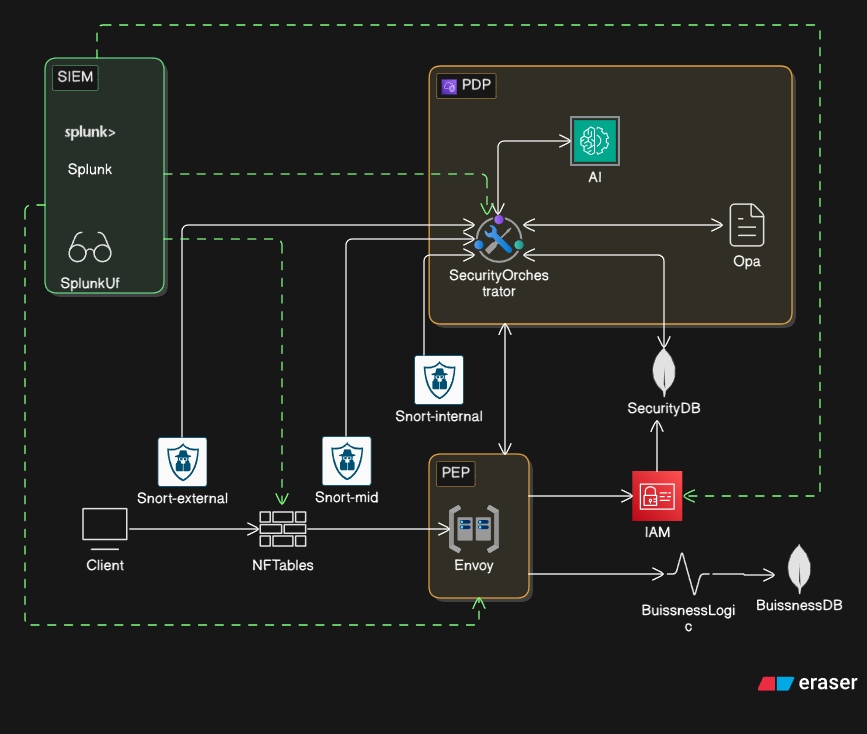
\includegraphics[width=0.7\textwidth]{immagini/architettura.png}
    \caption{Immagine architettura}
    \label{fig:immagine}
\end{figure}

\section{Struttura della repository}

Il codice sorgente dell'infrastruttura è strutturato per rispecchiare la scomposizione logica del sistema. Le cartelle principali che compongono il progetto sono descritte nell'elenco seguente:

\begin{itemize}
\item \texttt{api/}: ospita il contratto protocollare \texttt{ext\_authz.proto}, che costituisce la definizione formale dell'interfaccia di comunicazione tra i sistemi;

\item \texttt{certs/}: raccoglie i certificati digitali e le chiavi private impiegati per la mutua autenticazione del canale cifrato, includendo i certificati della Certificate Authority interna e lo script di generazione \texttt{gen-certs.sh};

\item \texttt{deployments/}: racchiude le configurazioni per il deployment dell'infrastruttura, suddividendosi in \texttt{docker/}, che contiene il file \texttt{docker-compose.yaml} per l'avvio ordinario e \texttt{docker-compose.test.yaml} per i test, e \texttt{kubernetes/}, che contiene le definizioni per l'orchestrazione dei pod;

\item \texttt{docs/}: contiene la documentazione tecnica e le guide di riferimento per l'attivazione e la manutenzione dell'infrastruttura;

\item \texttt{infra/}: ospita i file di configurazione dei servizi infrastrutturali, strutturandosi in \texttt{databases/} per MongoDB, \texttt{envoy/} per il proxy, \texttt{nftables/} per il firewall, \texttt{opa/} per le regole di accesso e \texttt{snort/} con \texttt{snort-internal/} per il rilevamento delle intrusioni;

\item \texttt{services/}: comprende le implementazioni software dei servizi attivi, includendo \texttt{business-logic/} scritto in Go per la gestione dei dati applicativi, \texttt{frontend/} con le pagine statiche e l'interfaccia utente, e \texttt{security-orchestrator/} scritto in Go come coordinatore decisionale;

\item \texttt{tasks/}: contiene script e automazioni per l'esecuzione di operazioni periodiche e di manutenzione sul sistema;

\item \texttt{tests/}: raccoglie gli strumenti per la convalida dei componenti, comprendendo la cartella \texttt{clients/} con simulatori in Python e Go per la generazione di traffico e la cartella \texttt{dashboard-app/} per la visualizzazione dei log;

\item \texttt{tools/}: ospita utilità di supporto tra cui il seeder del database per la generazione di record coerenti.
\end{itemize}

La radice della repository ospita il file \texttt{.env} con le chiavi di configurazione necessarie, il file \texttt{.gitignore} e il file \texttt{README.md}.

\section{La segmentazione di rete}

La topologia di rete si articola in tre segmenti Docker isolati, applicando il controllo degli accessi a livello infrastrutturale. Questa compartimentazione assicura che un compromesso su un servizio non si propaghi ad altri domini.

La \texttt{Front-Net} rappresenta l'unico canale rivolto all'esterno. In questo segmento risiedono il firewall di rete, il proxy Envoy e il Security Orchestrator. Qualsiasi richiesta in ingresso deve attraversare questo canale, venendo sottoposta ai controlli del firewall prima di poter raggiungere i servizi interni.

La \texttt{Auth-Net} costituisce il segmento privato dedicato alla determinazione delle autorizzazioni. In questa rete cooperano il Security Orchestrator, il motore Open Policy Agent e il database di sicurezza. Il Security Orchestrator funge da unico elemento di connessione tra la \texttt{Front-Net} e la \texttt{Auth-Net}, impedendo la raggiungibilità diretta del database di sicurezza e del motore delle regole da parte dei client esterni.

La \texttt{Back-Net} è una rete protetta e riservata che unisce esclusivamente il servizio di business logic al relativo database di produzione. Questa separazione assicura che il database contenente i dati sensibili della centrale sia isolato sia dall'esterno sia dallo stesso piano di decisione delle policy, riducendo l'esposizione a tentativi di esfiltrazione. Il servizio Business Logic appartiene sia alla \texttt{Back-Net} sia alla \texttt{Auth-Net}, il che consente di esporre l'endpoint interno \texttt{/internal/session} al Security Orchestrator per l'arricchimento del contesto di autorizzazione, senza però esporre il database sottostante.

\section{Il firewall e il punto di ingresso}

Il container denominato \texttt{firewall} costituisce la barriera iniziale per il traffico in ingresso. Configurato tramite nftables su una distribuzione Alpine Linux, il firewall adotta una politica predefinita di tipo DROP per le catene di ingresso, transito e uscita.

Per impedire che il traffico possa aggirare i controlli, il proxy Envoy e i sistemi di rilevamento delle intrusioni Snort condividono lo stack di rete del firewall tramite la configurazione \texttt{network\_mode} di Docker. Questa unione assicura che ogni pacchetto debba superare i controlli a livello kernel prima di essere intercettato da Envoy o ispezionato da Snort.

La configurazione del firewall include regole per contrastare gli attacchi volumetrici di tipo SYN flood tramite una struttura dinamica denominata \texttt{syn\_meter}, la quale limita a venti pacchetti al secondo la frequenza per ogni indirizzo IP sorgente, respingendo le eccedenze con il log di avviso \texttt{fw-syn-flood-drop}. Inoltre, la catena di uscita implementa un filtraggio rigoroso che consente le sole comunicazioni dirette alle porte TCP di risoluzione dei nomi e ai microservizi interni, ossia le porte \texttt{53}, \texttt{8080}, \texttt{8081} e \texttt{8082}, scartando ogni altra richiesta in uscita sotto il log \texttt{fw-egress-drop}. Il demone \texttt{ulogd} raccoglie questi eventi tramite NFLOG e li scrive su un file in emulazione syslog. Un parser scritto in Go legge questo file e genera un log JSONL strutturato nel percorso \texttt{/var/log/ztaleaks/nftables/firewall.jsonl}, rendendolo disponibile per l'inoltro e l'indicizzazione centralizzata.

\section{Envoy Proxy come Policy Enforcement Point}

Il proxy Envoy agisce come Policy Enforcement Point del sistema, operando sulla porta \texttt{8443}. Il listener impiega il filtro \texttt{tls\_inspector} per analizzare l'handshake in modo precoce, estraendo l'impronta JA3 del client e rendendola disponibile nei metadati di sessione.

Il canale TLS è configurato per richiedere la presentazione facoltativa di un certificato client, demandando la verifica del possesso e la validazione del certificato al livello applicativo. Envoy utilizza il filtro HTTP \texttt{ext\_authz} configurato tramite il blocco \texttt{http\_service} per inoltrare in modo sincrono i dettagli della richiesta al Security Orchestrator sull'endpoint \texttt{/api/v1/evaluate} tramite una chiamata HTTP. La direttiva \texttt{failure\_mode\_allow} è impostata su \texttt{false}, applicando una modalità di blocco a fronte di un eventuale guasto del coordinatore.

Le informazioni estratte dal certificato client e l'impronta JA3 vengono inserite negli header \texttt{x-forwarded-client-cert} e \texttt{x-ja3-fingerprint} prima di inviare la richiesta all'orchestratore. I log di accesso di Envoy sono scritti in formato JSONL includendo il valore letterale \texttt{service: "envoy"}, mentre i campi relativi a punteggi di rischio esterni o identificativi di zona geografica sono momentaneamente omessi in quanto non popolati dalle logiche attuali del sistema.

\section{Il Security Orchestrator come Policy Administrator}

Il Security Orchestrator opera come Policy Administrator, ricevendo le richieste di valutazione dal proxy Envoy. Questo microservizio, sviluppato in Go, espone un server HTTP sulla porta \texttt{8081} e coordina le componenti coinvolte nel processo decisionale.

All'avvio, il servizio configura un logger JSON strutturato che integra il valore \texttt{service: "security-orchestrator"}. Per ogni richiesta ricevuta sulla rotta \texttt{/api/v1/evaluate}, l'orchestratore esegue le seguenti attività:

\begin{itemize}
\item estrae il token JWT dall'header di autorizzazione e ne convalida la firma crittografica tramite l'endpoint JWKS esposto dall'identity service;

\item identifica il dispositivo analizzando l'header del certificato mTLS e interroga il database di sicurezza per verificare la validità dell'attestazione TPM associata al dispositivo;

\item esegue un controllo in modalità trasparente, denominata Shadow Mode, confrontando l'unità organizzativa del certificato con il ruolo dell'utente ed evidenziando eventuali disallineamenti;

 \item arricchisce il contesto con il punteggio di rischio calcolato da un modello di
  Intelligenza Artificiale di tipo Temporal Graph Network (TGN), interrogato come microservizio
  esterno: il modello ricostruisce il grafo storico delle interazioni e restituisce un
  \textit{anomaly score} continuo nell'intervallo $[0,1]$. Per resistere ad attacchi di tipo
  \textit{poisoning}, l'interrogazione segue un flusso in due fasi: l'orchestratore chiama prima
  l'endpoint \texttt{/infer} in sola lettura per ottenere lo score e, solo se la decisione
  finale di OPA è di consenso, conferma l'evento nella memoria del modello tramite l'endpoint
  \texttt{/update}, così che gli accessi negati non contribuiscano mai all'addestramento. In
  caso di indisponibilità o timeout del servizio (cinque secondi), l'orchestratore adotta in
  modo conservativo uno score elevato pari a $0.99$ con confidenza \texttt{low}, traducendo
  l'incertezza in una postura più restrittiva;

\item compone un documento strutturato e interroga il motore OPA per la decisione definitiva.
\end{itemize}

Le decisioni emesse vengono registrate in un log dedicato denominato \texttt{opa\_decision.jsonl} per finalità di ispezione e analisi forense.

\subsection{Alert provenienti dagli Snort}

  Parallelamente al flusso di valutazione sincrono, il Security Orchestrator mantiene una cache
  in memoria degli alert generati dalle istanze Snort. Un listener TCP dedicato, in ascolto
  sulla porta \texttt{9000}, riceve dal parser degli IDS gli allarmi serializzati come JSON
  newline-delimited e li indicizza per indirizzo IP sorgente. Per ciascun IP la cache conserva
  tre slot distinti, corrispondenti alle istanze \textit{edge} (\texttt{snort}), \textit{mid}
  (\texttt{snort-mid}) e \textit{internal} (\texttt{snort-internal}), associati a una scadenza
  temporale (TTL) di tre minuti che viene rinnovata a ogni nuovo allarme. Al momento della
  valutazione di una richiesta, l'orchestratore interroga la cache per l'IP del client e
  converte la presenza di allarmi recenti in feature binarie, passate al modello TGN insieme
  agli altri attributi della richiesta (corrispondenza del fingerprint JA3, metodo, ruolo e
  livello di clearance). In questo modo un'attività di rete sospetta rilevata da Snort innalza
  in tempo reale lo score di rischio associato alle richieste provenienti dal medesimo
  indirizzo, senza introdurre latenza aggiuntiva nel percorso decisionale.

\section{OPA come Policy Decision Point}

La policy predefinita applica un approccio \textit{default deny}, bloccando qualsiasi richiesta non esplicitamente autorizzata. La valutazione autorizzativa si articola ad alto livello su una catena di controlli logici sequenziali: la verifica di eventuali esenzioni per le rotte pubbliche, l'assegnazione degli attributi di sicurezza in base all'identità (RBAC), la validazione matematica dell'appartenenza ai compartimenti richiesti (Categorie) e il controllo gerarchico di confidenzialità basato sulle direttive del modello Bell-LaPadula.

A valle dei controlli strutturali, la policy integra la valutazione continua del rischio generata in tempo reale dai sistemi di Intelligenza Artificiale. Invece di affidarsi a soglie di blocco fisse o a meccanismi di fallback statici, il sistema valuta ogni singola transazione attraverso il calcolo di un bilancio di rischio netto: l'accesso viene definitivamente autorizzato solo se il beneficio intrinseco dell'operazione, decurtato dello score di minaccia calcolato dall'AI, risulta superiore al livello di rischio accettato per quello specifico endpoint.


\section{Il Business Logic service}

Il servizio Business Logic rappresenta il backend applicativo che gestisce il dominio operativo della centrale. Il servizio è scritto in Go e popola i propri log integrando il campo \texttt{service: "business-logic"} per abilitare la correlazione automatica in Splunk.

Un middleware intercetta le richieste in transito, estraendo gli header di tracciamento iniettati da Envoy come \texttt{X-Request-ID}, \texttt{X-Current-User} e \texttt{X-Ja3-Fingerprint}. Questi dati vengono combinati con la durata e lo stato della risposta per produrre un record di log esaustivo.

Per garantire la protezione contro tentativi di manomissione diretta della base dati, il servizio implementa una convalida dell'integrità: all'atto della creazione o dell'aggiornamento di un record sensibile, il sistema calcola un hash SHA-256 concatenando i campi informativi con un carattere di separazione pipe; questo hash viene memorizzato nel documento e ricalcolato a ogni lettura, bloccando la visualizzazione e sollevando un errore qualora si rilevi una divergenza.

\section{Identity Access Management service}
Il servizio Identity Access Management (\texttt{iam-service}) gestisce l'intero ciclo di vita dell'autenticazione e dell'identità. È scritto in Go, espone un server HTTP sulla porta  \texttt{8082} e popola i propri log integrando il campo \texttt{service: "iam-service"} per la correlazione automatica in Splunk.
L'autenticazione segue un flusso a due fasi che incorpora un secondo fattore obbligatorio. Nella prima fase, la rotta \texttt{/api/v1/auth/login} verifica le credenziali confrontando la
password con un hash \texttt{Argon2id} e controlla il certificato client propagato da Envoy controllando il campo CN deve corrispondere allo username e l'unità organizzativa al ruolo dichiarato. Superati questi controlli, il servizio genera un codice OTP a sei cifre, ne
memorizza l'hash HMAC-SHA256 con una scadenza di cinque minuti e un massimo di tre tentativi,  e lo invia all'indirizzo email registrato. Nella seconda fase, la rotta  \texttt{/api/v1/auth/verify-otp} valida il codice e, solo in caso di esito positivo, rilascia
il token di sessione.
Il token emesso è un JWT firmato con algoritmo RS256, con chiave pubblica RSA corrispondente è pubblicata sull'endpoint  \texttt{/.well-known/jwks.json}, da cui il Security Orchestrator la recupera per verificare in  autonomia la firma di ogni token, senza dover condividere segreti con l'iam-service.

Il servizio gestisce inoltre l'elevazione del livello di fiducia del dispositivo. Attraverso le cerimonie WebAuthn/FIDO2  un utente può registrare un dispositivo tramite TPM: la credenziale viene salvata nella collezione \texttt{device\_fingerprints},

\section{I database}

L'infrastruttura utilizza due database MongoDB separati per impedire la commistione tra dati di sicurezza e informazioni di produzione.

Il Business DB memorizza i dati del personale e della centrale. Il database abilita l'autenticazione obbligatoria e definisce quattro utenze a minimo privilegio, assegnando permessi distinti per le operazioni di scrittura applicativa, per il caricamento iniziale dei dati, per il motore PDP e per i lettori di monitoraggio. Ciascuna delle sette collezioni è protetta da un JSON Schema che valida i tipi di dato e la coerenza dei formati. I documenti del personale e delle zone includono rispettivamente i sotto-documenti \texttt{ztna\_metadata} e \texttt{ztna\_policy} per supportare le verifiche del Policy Decision Point.

Il Security DB è destinato esclusivamente al salvataggio delle impronte digitali dei dispositivi registrati nella collezione \texttt{device\_fingerprints} e degli utenti abilitati nel servizio di identità, rimanendo accessibile solo all'orchestratore e al servizio di identità.

\section{Il sistema di rilevamento delle intrusioni}

Il monitoraggio della sicurezza di rete si avvale di tre istanze distinte di Snort, posizionate strategicamente all'interno dell'infrastruttura per ispezionare il traffico a diversi livelli:

\begin{itemize}
    \item \textbf{Istanza Esterna (\texttt{snort}):} Analizza il traffico in ingresso sulla \texttt{Front-Net} e si concentra sull'individuazione di scansioni di porte tramite il modulo \texttt{sfportscan}, rilevando attività sospette a fronte di cinque pacchetti SYN ravvicinati provenienti dal medesimo mittente.
    \item \textbf{Istanza Interna (\texttt{snort-internal}):} Analizza le transazioni interne dirette verso il proxy Envoy, cercando violazioni del canale TLS. Questo comprende l'individuazione di negoziazioni prive di certificato client, l'impiego di cifrari obsoleti o connessioni basate su versioni non sicure del protocollo.
    \item \textbf{Istanza Mid (\texttt{snort-mid}):} Ispeziona il traffico applicativo in transito tra Envoy e il Security Orchestrator (sul canale \texttt{ext\_authz}). Questa istanza è specificamente configurata per rilevare e segnalare vettori di attacco di livello 7, come tentativi di SQL Injection e Cross-Site Scripting (XSS).
\end{itemize}

\subsection{Meccanismo di Inoltro degli Alert}
Affinché le minacce vengano gestite tempestivamente, le istanze IDS sono collegate a un sistema di telemetria in tempo reale. Un parser personalizzato scritto in Go legge i log generati dalle tre istanze di Snort in modalità \textit{tailing}, normalizzandoli in formato JSONL. 

Una volta normalizzato, ogni evento critico viene immediatamente inoltrato al Security Orchestrator attraverso una connessione socket TCP diretta (sulla porta 9000). Questo scambio avviene su una porzione di rete privata dedicata esclusivamente al trasporto degli allarmi (\texttt{snort-net}). L'utilizzo del socket TCP permette un invio a bassissima latenza, garantendo che gli eventi di sicurezza raggiungano il motore decisionale centrale nel momento esatto in cui vengono rilevati sul livello di rete, pronti per l'indicizzazione e per innescare eventuali risposte di mitigazione.


\section{Il frontend}

L'interfaccia utente è costituita da un'applicazione web statica servita da Nginx. L'interfaccia comunica direttamente con l'API esposta da Envoy sulla porta \texttt{8443}.

Il frontend gestisce in modo autonomo il token di autenticazione e richiede un token CSRF prima di intraprendere operazioni di scrittura. Sebbene la sicurezza sia garantita dal controllo delle policy eseguito dal PDP, il frontend implementa regole lato client per nascondere o disattivare elementi grafici non conformi ai privilegi dell'utente, migliorando la qualità dell'interazione.

\section{Il seeder}

Il seeder è uno strumento sviluppato in Go per popolare il Business DB. Per garantire la coerenza, l'applicazione inserisce i record rispettando rigorosamente le dipendenze referenziali tra le collezioni.

Il seeder calcola preventivamente gli hash di integrità crittografica per i record inseriti, rendendo l'ambiente immediatamente verificabile e pronto all'uso fin dalla prima inizializzazione.

\section{Il flusso di autorizzazione end-to-end}

La cooperazione tra i componenti può essere compresa seguendo il percorso di una transazione, illustrato nella catena di passaggi descritta di seguito:

\begin{itemize}
\item il client effettua la chiamata verso la porta \texttt{8443} di Envoy, attraversando le regole del firewall che verificano l'assenza dell'indirizzo sorgente dalla lista nera e valutano i limiti di frequenza;

\item Envoy instaura la sessione TLS raccogliendo i dati del certificato client e l'impronta JA3, inviando poi una chiamata HTTP al Security Orchestrator con i dettagli della transazione;

\item il Security Orchestrator valida il token JWT tramite JWKS, verifica l'attestazione TPM sul database di sicurezza e arricchisce la richiesta con il punteggio del rischio calcolato dai sistemi di Intelligenza Artificiale;

\item OPA riceve l'input arricchito dall'orchestratore, valuta la policy multi-dimensionale e restituisce il verdetto finale;

\item se OPA consente l'accesso, l'orchestratore autorizza Envoy, il quale inoltra la richiesta al Business Logic; quest'ultimo convalida l'integrità dei record tramite SHA-256 e risponde al client includendo l'identificativo \texttt{X-Request-ID} per la correlazione centralizzata dei log.
\end{itemize}